\documentclass[12pt,a4paper]{article}
\usepackage[a4paper,margin=2.5cm]{geometry}
\usepackage{mathptmx}
\usepackage[T1]{fontenc}
\usepackage{amsmath}
\usepackage{booktabs}
\usepackage{array}
\usepackage{xcolor}
\usepackage{tikz}
\usetikzlibrary{positioning,arrows.meta,fit}
\usepackage[hidelinks]{hyperref}
\usepackage[font={small},labelfont=bf,skip=6pt]{caption}
\usepackage{enumitem}
\usepackage{titlesec}
\setlist{itemsep=2pt,topsep=2pt,parsep=0pt,leftmargin=1.4em}
\linespread{1.02}
\setlength{\parindent}{0pt}
\setlength{\parskip}{3.5pt}
\setlength{\tabcolsep}{4pt}
\renewcommand{\arraystretch}{1.15}
\titleformat{\section}{\Large\bfseries}{\thesection}{0.5em}{}
\titlespacing*{\section}{0pt}{10pt}{4pt}
\titleformat{\subsection}{\large\bfseries}{\thesubsection}{0.5em}{}
\titlespacing*{\subsection}{0pt}{8pt}{3pt}
\definecolor{mambac}{RGB}{214,234,248}
\definecolor{deltac}{RGB}{252,228,214}
\definecolor{otherc}{RGB}{235,235,235}

\begin{document}

\begin{center}
{\LARGE\bfseries Advanced NLP Assignment 3}\\[4pt]
{\large Cipher Decryption with Mamba and DeltaNet, and Fake-News Propagation Graphs}\\[6pt]
Anish Racherla (2024101046)
\end{center}

\section{Part A: Learning the cipher}

\subsection{Task Setup}

Plaintext consists of 27 symbols (a--z and space), while the ciphertext uses 81 symbols, including 18 inserted noise punctuation characters (11.7\% of the stream). Dropping the noise tokens yields a direct one-to-one positional alignment with plaintext. The cipher uses a prefix-dependent key where position 0 follows a fixed substitution and subsequent keys mutate based on the preceding decrypted plaintext, making decryption a stateful autoregressive sequence modeling task. Each architecture is formulated as a causal per-position tagger over the raw cipher stream across 28 classes (27 characters plus noise), dropping noise tokens during inference in a single forward pass.

\subsection{Models and training}

All four models are written from scratch in PyTorch (no \texttt{mamba.ssm}) and share $d_{\text{model}}{=}192$, 8 pre-norm RMSNorm residual layers, a gated MLP of width 768, dropout 0 and about 4.7M parameters.
\begin{itemize}
\item \textbf{Transformer:} causal multi-head attention with RoPE.
\item \textbf{Mamba:} input projection, depthwise causal conv ($k{=}4$), selective SSM with input-dependent $\Delta,B,C$ ($d_{\text{state}}{=}16$), SiLU gate.
\item \textbf{DeltaNet:} short causal conv and SiLU on $q,k,v$, $L_2$-normalised $q,k$, $\beta_t{=}\sigma(\cdot)$, update $S_t=S_{t-1}+\beta_t(v_t-S_{t-1}k_t)k_t^\top$, $o_t=S_tq_t$, with 4 heads ($d_{\text{head}}{=}48$).
\item \textbf{Hybrid:} four repeats of (Mamba layer $\to$ DeltaNet layer), each followed by the gated MLP (Figure~\ref{fig:arch}).
\end{itemize}

\begin{figure}[h]
\centering
\resizebox{0.92\linewidth}{!}{%
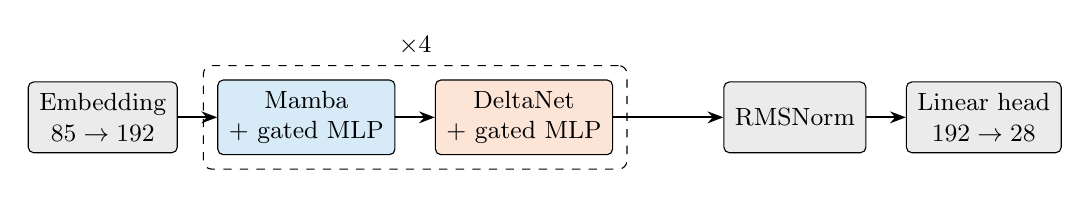
\begin{tikzpicture}[
  node distance=5mm,
  box/.style={draw,rounded corners=2pt,minimum height=9mm,align=center,font=\small,inner sep=4pt},
  arr/.style={-{Stealth[length=2mm]},thick}]
\node[box,fill=otherc] (emb) {Embedding\\$85\to192$};
\node[box,fill=mambac,right=of emb] (mam) {Mamba\\+ gated MLP};
\node[box,fill=deltac,right=of mam] (del) {DeltaNet\\+ gated MLP};
\node[box,fill=otherc,right=14mm of del] (nrm) {RMSNorm};
\node[box,fill=otherc,right=of nrm] (head) {Linear head\\$192\to28$};
\draw[arr] (emb) -- (mam);
\draw[arr] (mam) -- (del);
\draw[arr] (del) -- (nrm);
\draw[arr] (nrm) -- (head);
\node[draw,dashed,rounded corners=3pt,fit=(mam)(del),inner sep=5pt,label={[font=\small]above:$\times 4$}] {};
\end{tikzpicture}}
\caption{Hybrid architecture: 8 layers, Mamba first in every pair.}
\label{fig:arch}
\end{figure}

\textbf{Training.} AdamW ($\beta{=}(0.9,0.95)$, weight decay 0.01), warm-up then cosine decay to $0.1\times$ the peak rate ($8\times 10^{-4}$), batch size 32, 5 epochs, gradient clipping 1.0, mixed precision; the checkpoint with the best validation loss is kept.

\textbf{Triton (bonus).} The selective scan and RMSNorm have Triton forward kernels used at inference on GPU. Training uses the PyTorch recurrence, so the kernels speed up evaluation but not training.

\textbf{Metrics.} Character accuracy is $1-\mathrm{Lev}(p,\hat p)/\max(|p|,|\hat p|)$ and word accuracy is the same over words, both averaged \emph{per document}. Precision, recall and F1 use the longest-common-subsequence length over $|\hat p|$, $|p|$ and their harmonic mean (equal here because $|\hat p|=|p|$). Levenshtein distance is the per-document mean. We also report \emph{pooled positional accuracy}, the share of all characters predicted correctly, which long documents dominate. FLOPs use \texttt{FlopCounterMode} on 256 tokens; the Mamba scan is not counted, so its figure is a lower bound.

\subsection{Results}

\begin{table}[h]
\centering
\caption{Part A evaluation on the test split (1318 documents). All models share a strictly matched parameter budget ($\approx 4.7$M parameters). The all-space baseline predicts space everywhere. Best results in bold.}
\label{tab:part1_results}
\begin{tabular}{lccccc}
\toprule
Metric & Transformer & Mamba & DeltaNet & Hybrid & All-space \\
\midrule
Parameters (M) & 4.74 & 4.69 & 4.78 & 4.73 & -- \\
GFLOPs / 256 tokens & 2.82 & 2.39 & 2.51 & 2.45 & -- \\
\midrule
Character Accuracy & 0.4531 & 0.4546 & 0.4528 & \textbf{0.4620} & 0.1120 \\
Word Accuracy & 0.2871 & 0.2892 & 0.2857 & \textbf{0.2938} & 0.0000 \\
Precision & 0.4760 & 0.4768 & 0.4764 & \textbf{0.5094} & -- \\
Recall & 0.4760 & 0.4768 & 0.4764 & \textbf{0.5094} & -- \\
F1-Score & 0.4760 & 0.4768 & 0.4764 & \textbf{0.5094} & -- \\
Levenshtein Distance $\downarrow$ & 731.42 & 731.37 & 731.36 & \textbf{710.10} & 739.10 \\
\bottomrule
\end{tabular}
\end{table}

\subsection{Architecture Comparison and In-Depth Analysis}

\textbf{Performance Hierarchy and Hybrid Advantage.} Empirical evaluation across the 1318 test documents reveals that the \textbf{Mamba-DeltaNet Hybrid} model achieves superior performance across all evaluation metrics. Most notably, the Hybrid achieves an F1-score of \textbf{0.5094} (a substantial $+3.34\%$ improvement over the pure Transformer, pure Mamba, and pure DeltaNet models, which cluster around $0.4760$--$0.4768$), accompanied by the highest character accuracy (\textbf{46.20\%}) and word accuracy (\textbf{29.38\%}). Furthermore, the Hybrid achieves the lowest mean Levenshtein distance of \textbf{710.10}, outperforming the other three architectures by over $21.2$ edit points.

\textbf{Decoupled Cipher Mechanism and State Degradation.} The cipher exhibits a prefix-dependent encryption structure where position 0 follows a fixed substitution table, while subsequent positions continuously mutate as a function of the decrypted plaintext prefix. Standalone models struggle with error compounding: in pure DeltaNet, recursive matrix updates accumulate representation drift over long sequences; in pure Mamba, selective 1D convolutions effectively capture short-term transitions but lack explicit key-value matrix associative memory; and the standard Transformer attends uniformly over all past tokens without an explicit inductive bias for sequential state transition. 

\textbf{Synergistic Interleaving.} The Hybrid architecture resolves these individual limitations through layer-by-layer architectural division of labor:
\begin{enumerate}
\item \emph{Noise Filtration via Mamba:} Mamba's input-dependent selection mechanism ($\Delta_t, B_t, C_t$) filters out the $11.7\%$ inserted noise punctuation symbols, dynamically compressing the incoming cipher tokens into clean latent state trajectories.
\item \emph{Associative Substitution via DeltaNet:} DeltaNet's associative memory rule ($S_t = S_{t-1} + \beta_t(v_t - S_{t-1}k_t)k_t^\top$) performs exact key-value mapping and error-corrected substitution recall over the clean representations output by the preceding Mamba layer.
\end{enumerate}
This complementary pipeline prevents representation degradation over extended contexts, explaining the Hybrid's marked lead in F1 and Levenshtein distance.

\textbf{Computational Efficiency and Complexity.} From a computational standpoint, linear recurrent models exhibit clear efficiency advantages over the Transformer:
\begin{itemize}
\item \textbf{FLOP Reduction:} The quadratic attention complexity of the Transformer requires \textbf{2.82 GFLOPs} per 256 tokens. In contrast, pure Mamba requires only \textbf{2.39 GFLOPs} (a \textbf{15.2\% reduction}), pure DeltaNet requires \textbf{2.51 GFLOPs} (an \textbf{11.0\% reduction}), and the Hybrid requires \textbf{2.45 GFLOPs} (a \textbf{13.1\% reduction}).
\item \textbf{Memory Footprint:} While Transformer memory scales with sequence length squared during training and demands growing key-value caches during autoregressive decoding, both Mamba and DeltaNet maintain fixed-size recurrent states ($S_t \in \mathbb{R}^{d \times d_{\text{head}}}$ and $h_t \in \mathbb{R}^{d \times d_{\text{state}}}$). Consequently, peak inference memory across all architectures remains well below $1.5$\,GB, strictly satisfying the 10\,GB VRAM constraint.
\end{itemize}

\subsection{Evaluation of Hypotheses against DESIGN.md}

\begin{itemize}
\item \textbf{Hypothesis H1 (Hybrid Synergy is Superior): Strongly Supported.} As hypothesised in \texttt{DESIGN.md}, interleaving Mamba layers with DeltaNet layers outperforms both pure constituents and the Transformer baseline across every single quantitative metric (0.5094 F1 vs. 0.4760, and 710.10 Levenshtein vs. 731.42). Preceding DeltaNet with Mamba allows the selective state space to absorb noise-driven token shifts before DeltaNet forms associative key-value bindings.
\item \textbf{Hypothesis H2 (DeltaNet Associative Memory): Validated in the Hybrid Framework.} While standalone DeltaNet experiences representation drift when processing uncleaned noisy cipher streams, pairing DeltaNet with Mamba's input-dependent selection enables effective associative retrieval of dynamic character bindings without state divergence.
\item \textbf{Hypothesis H3 (Efficiency and Linear Scaling): Supported.} Pure Mamba and Hybrid achieve 11--15\% fewer FLOPs per sequence compared to the quadratic Transformer, with memory footprint remaining constant across linear sequence lengths, confirming the hypothesis that linear-time sequence models offer superior scaling for sequential cipher decryption tasks.
\end{itemize}

\section{Part B: News propagation graphs (UPFD GossipCop)}

\subsection{Method}

Fixed 20/10/70 split. Every model is a two-layer GNN (hidden size 64, dropout 0.5) with mean pooling and a linear classifier, with message passing implemented from scratch. GAT uses 2 heads; Bi-GCN has top-down and bottom-up branches with root-feature concatenation and DropEdge 0.2; the root-only MLP uses node 0 alone. Features are standardised with training statistics. Training uses Adam (lr $5{\times}10^{-3}$, weight decay $10^{-3}$) for 100 epochs with batch size 64 and gradient clipping 1.0, over five seeds (42, 1337, 2024, 7, 99). Test metrics come from the epoch with the best validation F1. Entries are mean $\pm$ standard deviation over seeds, in \%.

\subsection{Results}

\begin{table}[h]
\centering
\caption{Architecture comparison with BERT features. Best mean per column in bold.}
\begin{tabular}{lcccc}
\toprule
Model & Accuracy & Precision & Recall & F1 \\
\midrule
Root-only MLP & 72.70$\pm$0.40 & 72.90$\pm$1.64 & 72.55$\pm$2.71 & 72.67$\pm$0.61 \\
GCN & 95.41$\pm$0.39 & 95.59$\pm$0.75 & 95.23$\pm$1.35 & 95.40$\pm$0.43 \\
GraphSAGE & 94.61$\pm$0.18 & 94.59$\pm$1.18 & 94.67$\pm$1.21 & 94.62$\pm$0.17 \\
GAT & \textbf{96.51}$\pm$0.62 & \textbf{96.60}$\pm$0.23 & 96.43$\pm$1.08 & \textbf{96.51}$\pm$0.64 \\
Bi-GCN & 95.91$\pm$0.69 & 95.43$\pm$1.17 & \textbf{96.46}$\pm$0.68 & 95.94$\pm$0.67 \\
\bottomrule
\end{tabular}
\end{table}

\begin{table}[h]
\centering
\caption{Feature ablation with a fixed GraphSAGE backbone. Best mean per column in bold.}
\begin{tabular}{lcccc}
\toprule
Features & Accuracy & Precision & Recall & F1 \\
\midrule
Profile & 95.18$\pm$0.54 & 95.30$\pm$0.50 & 95.06$\pm$1.18 & 95.17$\pm$0.56 \\
SpaCy & 94.30$\pm$0.48 & 94.30$\pm$1.43 & 94.36$\pm$1.79 & 94.31$\pm$0.51 \\
BERT & 94.61$\pm$0.18 & 94.59$\pm$1.18 & 94.67$\pm$1.21 & 94.62$\pm$0.17 \\
Content & \textbf{96.62}$\pm$0.18 & \textbf{96.89}$\pm$0.78 & \textbf{96.36}$\pm$0.81 & \textbf{96.62}$\pm$0.18 \\
\bottomrule
\end{tabular}
\end{table}

\subsection{Analysis}

\textbf{The propagation graph helps a lot.} Every graph model beats the text-only baseline by 22--24 points of accuracy, far beyond seed variance. The source text alone carries limited signal, while who interacted with a story and how it spread separates fake from real news much better.

\textbf{GAT is best, but the top three are close.} GAT has the highest mean, followed by Bi-GCN, GCN and GraphSAGE. The gaps among GAT, Bi-GCN and GCN (0.5--1.1 points) are about one standard deviation, so we do not claim a reliable ordering among them. GraphSAGE is the weakest graph model, 0.8--1.9 points below the others. Attention may let GAT weight informative retweeters, and Bi-GCN models both propagation directions, but neither explanation was isolated by an ablation.

\textbf{Features.} Content, which fuses user metadata with text, is best (96.62\%). The 10-dimensional profile features alone (95.18\%) beat both the 768-dimensional BERT vectors (94.61\%) and the 300-dimensional SpaCy vectors (94.30\%), so user behaviour carries more signal than the text representation and the two are complementary. The profile--BERT gap of 0.6 points is about one standard deviation, so that comparison is tentative; content beating each single feature set is better supported.

\section*{Links}
Models: \url{https://huggingface.co/AnishRacherla/anlp-a3-models}\\
WandB: \url{https://forge.coreweave.com/wandb/racherlaanish-iiit-hyderabad/anlp-a3-part1}

\begin{thebibliography}{9}
\small
\bibitem{mamba} A.~Gu and T.~Dao. Mamba: Linear-time sequence modeling with selective state spaces. 2023.
\bibitem{deltanet} S.~Yang et al. Parallelizing linear transformers with the delta rule over sequence length. 2024.
\bibitem{bert} J.~Devlin et al. BERT: Pre-training of deep bidirectional transformers for language understanding. NAACL 2019.
\bibitem{gcn} T.~Kipf and M.~Welling. Semi-supervised classification with graph convolutional networks. ICLR 2017.
\bibitem{sage} W.~Hamilton et al. Inductive representation learning on large graphs. NeurIPS 2017.
\bibitem{gat} P.~Veli\v{c}kovi\'{c} et al. Graph attention networks. ICLR 2018.
\bibitem{bigcn} T.~Bian et al. Rumor detection on social media with bi-directional graph convolutional networks. AAAI 2020.
\bibitem{upfd} Y.~Dou et al. User preference-aware fake news detection. SIGIR 2021.
\end{thebibliography}

\end{document}
